\newpage
\section{Ergebnisse}
In diesem Kapitel werden die zentralen Ergebnisse der Arbeit präsentiert.
Im Mittelpunkt steht der entwickelte \acs{aas}-Demonstrator, der die prototypische Umsetzung des digitalen Zwillings des Abfüll- und Verschließmoduls der robocell-Linie zeigt.
Darauf folgt die Analyse des eingesetzten Autoencoder-Modells zur Anomalieerkennung sowie die Vorstellung der beiden Anwendungsfälle \acs{dpp} und automatisierte Generierung der \acs{aas}.
Abschließend werden die im Projekt eingesetzten Softwarelösungen und Tools evaluiert.

\subsection{AAS-Demonstrator für die robocell}
\label{sec:AAS-Demonstrator}
Der \acs{aas}-Demonstrator basiert auf dem standardisierten Konzept der \acs{aas}.
Als zentrale Laufzeitumgebung kommt die Eclipse BaSyx-Plattform zum Einsatz, während für die Datenanbindung standardisierte Protokolle wie OPC~UA sowie HTTP/REST verwendet werden.
Der Demonstrator umfasst neben der Haupt-AAS der robocell-Maschine auch exemplarische AAS untergeordneter Komponenten, wodurch eine modulare und hierarchisch aufgebaute digitale Repräsentation entsteht.

Im weiteren Verlauf wird zunächst die Architektur des Gesamtsystems vorgestellt.
Sie dient der Verwaltung und Bereitstellung aller modellierten \acs{aas} und bildet die Grundlage für die dynamische Erweiterung um Echtzeit- und Zeitreihendaten.
Anschließend werden die im Demonstrator abgebildeten Aspekte der Maschine beschrieben, gegliedert in statische und dynamische Submodelle.
Den Abschluss bildet eine kurze Reflexion über zentrale Herausforderungen, die während der Implementierung aufgetreten sind.

\subsubsection{Systemarchitektur}
Die eingesetzte Architektur besteht aus mehreren Komponenten, die gemeinsam einen aktiven digitalen Zwilling im Sinne einer Typ-2-\acs{aas} ermöglichen.
Sie basiert vollständig auf containerisierten Diensten, die innerhalb einer gemeinsamen Docker-Umgebung über ein gemeinsames Netzwerk miteinander kommunizieren.
Dadurch entsteht eine modulare, skalierbare Infrastruktur, die sich flexibel erweitern und an veränderte Anforderungen anpassen lässt.

Als zentrale Plattform zur Bereitstellung und Verwaltung der \acs{aas} dient Eclipse BaSyx.
Ursprünglich war der Einsatz des AASX Server Blazor vorgesehen, dieser wurde jedoch frühzeitig durch BaSyx ersetzt, da sie eine deutlich flexiblere und funktionsreichere Umgebung für die Umsetzung digitaler Zwillinge bietet.
Abbildung~\ref{fig:BaSyxArchitektur} zeigt den Aufbau des zugrundeliegenden Systems, das als zentrales BaSyx-Backend die Verwaltung aller AAS-Komponenten übernimmt.

\begin{figure}[htbp]
    \centering
        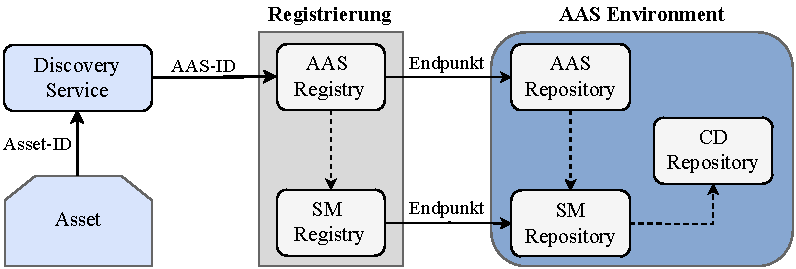
\includegraphics[width=1\textwidth]{Bilder/Ergebnisse/Systemarchitektur/BaSyx.pdf}
    \caption{BaSyx-Backend}
    \label{fig:BaSyxArchitektur}
\end{figure}

Der Discovery Service übernimmt die Auflösung einer Asset-ID (globalAssetId) in die zugehörige \acs{aas}-ID und ermöglicht so das gezielte Auffinden einer \acs{aas} im Gesamtsystem. 
Die Registries dienen als Verzeichnisse aller registrierten \acs{aas} und Submodelle einschließlich ihrer Endpunkte innerhalb der \acs{aas} Environment, wobei die \acs{aas} Registry optional auch Referenzen auf die Submodel Registry (SM Registry) enthalten kann. 

Die \acs{aas} Environment selbst beherbergt die eigentlichen Inhalte und ist in drei Repositories gegliedert. 
Das AAS Repository verwaltet die \acs{aas} einschließlich Asset-Metadaten und Referenzen auf Submodelle. 
Das Submodel Repository (SM Repository) speichert die Submodelle mit ihren jeweiligen Inhalten und Referenzen auf die zugehörigen Concept Descriptions. 
Diese werden im \acs{cd} Repository verwaltet und beeinhalten alle semantischen Beschreibungen.

Alle Komponenten verfügen dabei über eine standardisierte REST-API, die sowohl anderen Systemen als auch den Komponenten selbst einen einheitlichen Zugriff auf ihre Inhalte ermöglicht. 
Zudem sind sie an eine gemeinsame MongoDB angebunden, in der sämtliche Daten persistent gespeichert werden.

Die dynamische Erweiterung ergänzt die Kernarchitektur um die Fähigkeit zur Verarbeitung von Echtzeit- und Zeitreihendaten. 
Abbildung~\ref{fig:DynamischeErweiterungArchitektur} zeigt den Aufbau der zusätzlichen Komponenten sowie deren Zusammenspiel mit dem bestehenden System.

Der Datengenerator und der Maschinensimulator simulieren die robocell-Maschine und erzeugen sowohl Zustands- als auch kontinuierlich Prozessdaten. 
Beide Anwendungen stellen ihre Daten über einen OPC UA Server bereit und sind über die Databridge direkt an die AAS Environment im BaSyx-Backend angebunden.
Zusätzlich werden die vom Datengenerator simulierten Werte mithilfe von Telegraf kontinuierlich in eine InfluxDB geschrieben, wodurch eine historische Datenbasis entsteht. 

\begin{figure}[htbp]
    \centering
        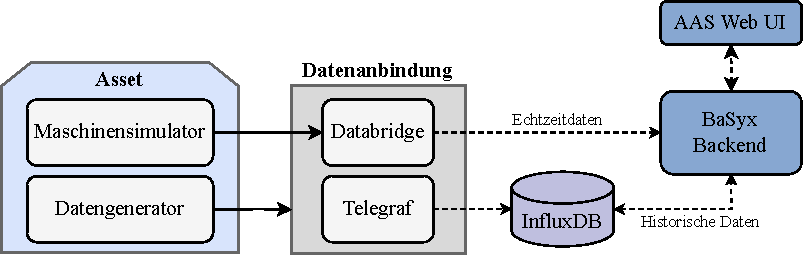
\includegraphics[width=1\textwidth]{Bilder/Ergebnisse/Systemarchitektur/DynamischeErwweiterung.pdf}
    \caption{BaSyx Backend}
    \label{fig:DynamischeErweiterungArchitektur}
\end{figure}

Zur Weiterverarbeitung und Visualisierung, sowohl der statischen Inhalte der AAS als auch der durch die dynamische Erweiterung ergänzten Echtzeit- und Zeitreihendaten, kommt die AAS Web UI zum Einsatz. 
Alternativ könnten auch benutzerdefinierte Anwendungen verwendet werden, die beispielsweise zusätzliche Analysen ermöglichen oder spezifische Anforderungen erfüllen.

Die AAS Web UI greift über die standardisierten Schnittstellen der Komponenten des zuvor vorgestellten BaSyx-Backends auf die Registrierungsdaten der AAS sowie deren Submodelle und Inhalte zu. 
Statische Daten und Echtzeitdaten werden dabei direkt aus dem Submodel Repository abgefragt. 
Bei Zeitreihendaten hingegen ist nicht der eigentliche Dateninhalt in der AAS gespeichert, sondern lediglich ein Verweis auf den zugehörigen Endpunkt in der InfluxDB hinterlegt. 
Die AAS Web UI nutzt diesen Endpunkt, um die historischen Daten direkt aus der Datenbank abzurufen und in der Web-Oberfläche zu visualisieren.

\subsubsection{Statische Submodelle}
Die statische Modellierung des Demonstrators erfolgte im Package Explorer.
Dazu wurden alle relevanten AAS sowie die zugehörigen Submodelle angelegt, mit Inhalten befüllt, semantisch angereichert und mit eindeutigen Identifikatoren versehen.
Als Hauptdatenquellen dienten die technischen Dokumentationen der robocell, insbesondere die Betriebsanleitung, sowie Informationen aus dem PLM-System Agile.

Abbildung~\ref{fig:PackageExplorerRobocell} zeigt die Gesamtübersicht des Abfüll- und Verschließmoduls. 
Die statischen Submodelle sind darin mit einer Nummer gekennzeichnet, die der im Folgenden verwendeten Gliederung entspricht. 
Sie beinhalten feststehende, beschreibende Inhalte, die nicht zur Laufzeit geändert werden. 
Zur besseren Veranschaulichung wird das Submodell BOM ausführlicher beschrieben.
Die grundlegende Struktur der weiteren statischen Submodelle ist im Anhang~\ref{sec:AnhangSubmodelle} ergänzend anhand von Screenshots dokumentiert.

\begin{figure}[htbp]
    \centering
        \includegraphics[width=1\textwidth]{Bilder/ErgebnissePackageExplorer/AASrobocellTestAuflösung.PNG}
    \caption{Package Explorer: Gesamtübersicht AAS-Demonstrator}
    \label{fig:PackageExplorerRobocell}
\end{figure}

\subsubsection*{1) Typenschild}
\vspace{-0.5em} 
Das Submodell Typenschild bildet die zentrale Identifikationsstelle der Maschine innerhalb der AAS. 
Es erfasst grundlegende Angaben wie Hersteller, Seriennummer, Produkttyp oder Softwareversionen. 
Funktional entspricht es einem physischen Typenschild, erweitert dieses jedoch um maschinenlesbare und interoperable Inhalte. 
Darüber hinaus bietet es den Vorteil, dass auch zusätzliche Dateien wie Zertifikate oder Logos direkt eingebunden werden können.

\subsubsection*{2) Technische Daten}
\vspace{-0.5em}

Das Submodell Technische Daten dient als technisches Datenblatt der Maschine.  
Es gliedert sich in die Bereiche Allgemeine Informationen sowie Technische Eigenschaften. 
Letztere sind in mehreren \acsp{smc} organisiert, beispielsweise für Produktionsmedien, Umgebungsbedingungen, elektrische Daten oder den Verarbeitungsbereich. 
Die einzelnen \acsp{smc} enthalten überwiegend Properties oder Ranges, die Parameter wie etwa elektrische Kenndaten beschreiben. 
Auf diese Weise sind alle relevanten technischen Angaben an einem zentralen Ort gebündelt, was der redundanten Pflege in verschiedenen Systemen oder Dokumenten entgegenwirkt. 

\subsubsection*{3) BOM}
\vspace{-0.5em}

Das BOM-Submodell dient dazu, die Maschinenstruktur sichtbar zu machen und die Beziehungen zwischen ihren einzelnen Komponenten hierarchisch abzubilden, vergleichbar mit einer digitalen Stückliste.
Dabei enthält es verschiedene Entitäten, die jeweils eine untergeordnete Komponente repräsentieren.
Die Beziehungen zwischen den Komponenten werden über Relationship-Elemente mit einer eindeutigen semanticId gemäß dem \acs{smt} Hierarchical Structures enabling Bills of Material \cite{SpezifikationHierachischeStrukturen} hergestellt.

Zur Veranschaulichung wurde die Grundmaschine als Beispiel gewählt, da sie weniger komplex als die Maschinenebene ist, aber dennoch alle relevanten Strukturelemente enthält.
Abbildung~\ref{fig:BOMSubmodelGrundmashcine} zeigt das entsprechende Submodell, in dem weitere untergeordnete Komponenten aufgeführt sind, darunter auch das Bedientableau.
Dieses ist als Self-Managed Entity angelegt und über die globalAssetId mit seiner AAS verknüpft (Abbildung~\ref{fig:AASBedientableau}), die wiederum ein eigenes BOM-Submodell mit weiteren Unterkomponenten enthält.

\begin{figure}[htbp]
    \centering
        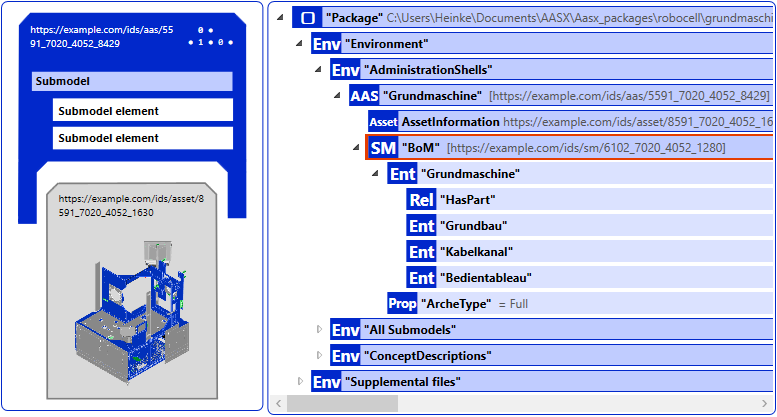
\includegraphics[width=1\textwidth]{Bilder/ErgebnissePackageExplorer/AASGrundmaschine.PNG}
    \caption{Package Explorer: BOM-Submodell der Grundmaschine}
    \label{fig:BOMSubmodelGrundmashcine}
\end{figure}

\begin{figure}[htbp]
    \centering
        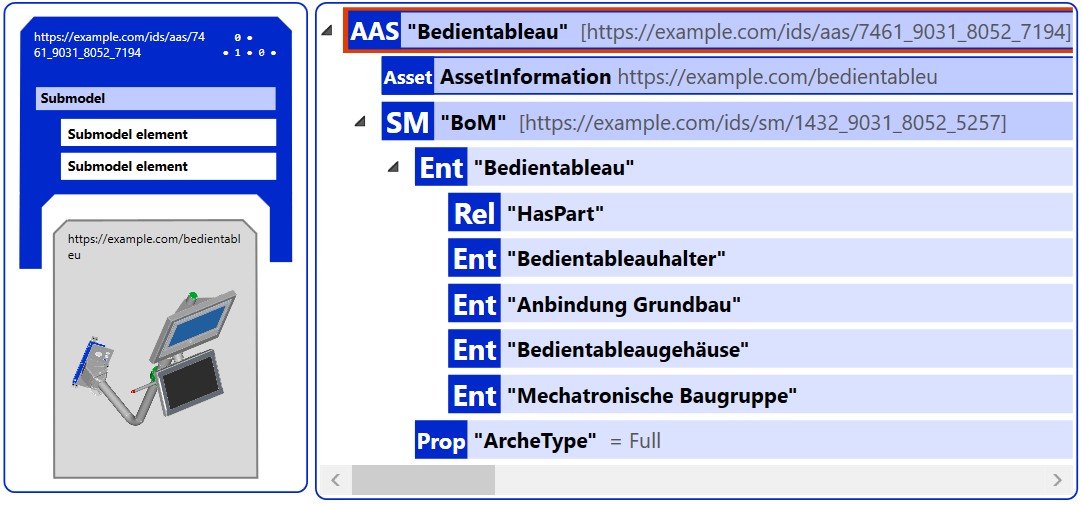
\includegraphics[width=1\textwidth]{Bilder/ErgebnissePackageExplorer/BedientableauTest.PNG}
    \caption{Package Explorer: AAS des Bedientableaus}
    \label{fig:AASBedientableau}
\end{figure}


Mit diesem Prinzip lässt sich die gesamte Maschine rekursiv abbilden. 
Jede Komponente wird als eigenständige AAS geführt und ist somit unabhängig von der übergeordneten Struktur wiederverwendbar. 
Dies ermöglicht eine modulare und herstellerübergreifende Integration, da auch externe Komponenten eingebunden werden können.

\subsubsection*{4), 5) Dokumentation und 3D-Modelle}
\vspace{-0.5em}

Beide Submodelle dienen der Bereitstellung und Klassifizierung zentraler Maschinendateien. 
Das Submodell Dokumentation umfasst technische Unterlagen wie die Betriebsanleitung oder die Netzwerkübersicht, während das Submodell 3D-Modelle CAD-Daten zur Geometrie beeinhaltet. 
Alle Dateien sind als File-Elemente direkt in die Struktur der AAS eingebettet und jeweils in eigenen \acsp{smc} organisiert, die zusätzlich Metainformationen zu Identifikation, Klassifikation und Versionierung enthalten. 
Das Submodell 3D-Modelle könnte darüber hinaus um weitere Metadaten, etwa zu Darstellungsoptionen oder Geometrieinformationen, ergänzt werden, was im Demonstrator jedoch nicht umgesetzt wurde. 
Dadurch ermöglichen beide Submodelle nicht nur das Einbetten von Dateien, sondern auch deren eindeutige Beschreibung und Rückverfolgbarkeit über den gesamten Lebenszyklus hinweg.

\subsubsection*{6) Wartung}
Das Submodell Wartung bildet den digitalen Wartungsplan der Maschine ab. 
Für jede wartungsrelevante Komponente sind in eigenen \acsp{smc} letzte Wartungszeitpunkte, Intervalle, zuständige Personen oder Organisationen sowie die vorgesehenen Maßnahmen hinterlegt. 
Es ermöglicht damit die strukturierte Verwaltung sowohl bereits durchgeführter als auch anstehender Wartungen und gewährleistet eine nachvollziehbare Dokumentation. 
Darüber hinaus schafft das Submodell die Grundlage für eine dynamische Erweiterung. 
So könnte beispielsweise ein Betriebsstundenzähler angebunden werden, der automatisch Wartungsbedarf erkennt, oder es könnte in Kombination mit Predictive-Maintenance-Ansätzen genutzt werden, um auf Basis von Sensordaten proaktiv Wartungsmaßnahmen abzuleiten und diese direkt in der AAS darzustellen. 

\textbf{Zusammenfassung}  

Die statischen Submodelle bündeln alle relevanten Stammdaten der Maschine zentral an einem Ort. 
Dadurch wird eine einfache Weitergabe der Informationen entlang der Wertschöpfungskette ermöglicht. 
So kann die AAS beispielsweise in Form einer AASX-Datei an einen Betreiber übergeben werden, der direkten Zugriff auf die Daten benötigt. 
Ebenso können AAS einzelner Komponenten nahtlos in den digitalen Zwilling der Gesamtmaschine integriert werden. 
Durch die Orientierung an standardisierten \acsp{smt} und die semantische Beschreibung sind die Inhalte zudem interoperabel und können von unterschiedlichen Systemen oder Personen gleichermaßen interpretiert und genutzt werden. 

\subsubsection{Dynamische Submodelle}
\label{sec:DynamischeSubmodelle}
Neben den statischen Submodellen wurden im Demonstrator auch dynamische Submodelle umgesetzt.
Sie ermöglichen die kontinuierliche Erfassung und Aktualisierung von Maschinen- und Prozessdaten sowie die Interaktion mit dem zugrunde liegenden Asset.
Da im Rahmen dieser Arbeit keine reale Maschine zur Verfügung stand, wird dieses Asset durch den Datengenerator und den Maschinensimulator repräsentiert.

Die technische Umsetzung und die zugrunde liegenden Datenflüsse orientieren sich an etablierten Industriearchitekturen, sodass die Schnittstellen und Funktionsweisen ohne Anpassungen auch mit einem realen System genutzt werden könnten.
Durch diese Erweiterung erfüllt der Demonstrator die Anforderungen an einen digitalen Zwilling gemäß der in Kapitel~\ref{sec: DT} beschriebenen Klassifizierung.

\subsubsection*{Prozessdaten}

Das Submodell Prozessdaten dient der Erfassung und Bereitstellung zentraler Betriebsinformationen.
Im Rahmen dieser Arbeit wurden exemplarisch die Messgrößen Füllstand, Durchfluss, Anzahl abgefüllter Einheiten und Druck implementiert.
Die Werte stammen aus dem \acs{opcua}-Server des Datengenerators, der sie im Sekundentakt aktualisiert und über die Databridge nahezu in Echtzeit an die \acs{aas} überträgt.
Vor der Speicherung im Submodel Repository erfolgt eine zweistufige Transformation.
Zunächst werden die Rohdaten mithilfe des Jackson-Transformers in ein JSON-Format überführt, anschließend extrahiert JSONata die relevanten Messgrößen, die schließlich den entsprechenden Properties des Submodells zugeordnet werden.

\begin{figure}[htbp]
    \centering
    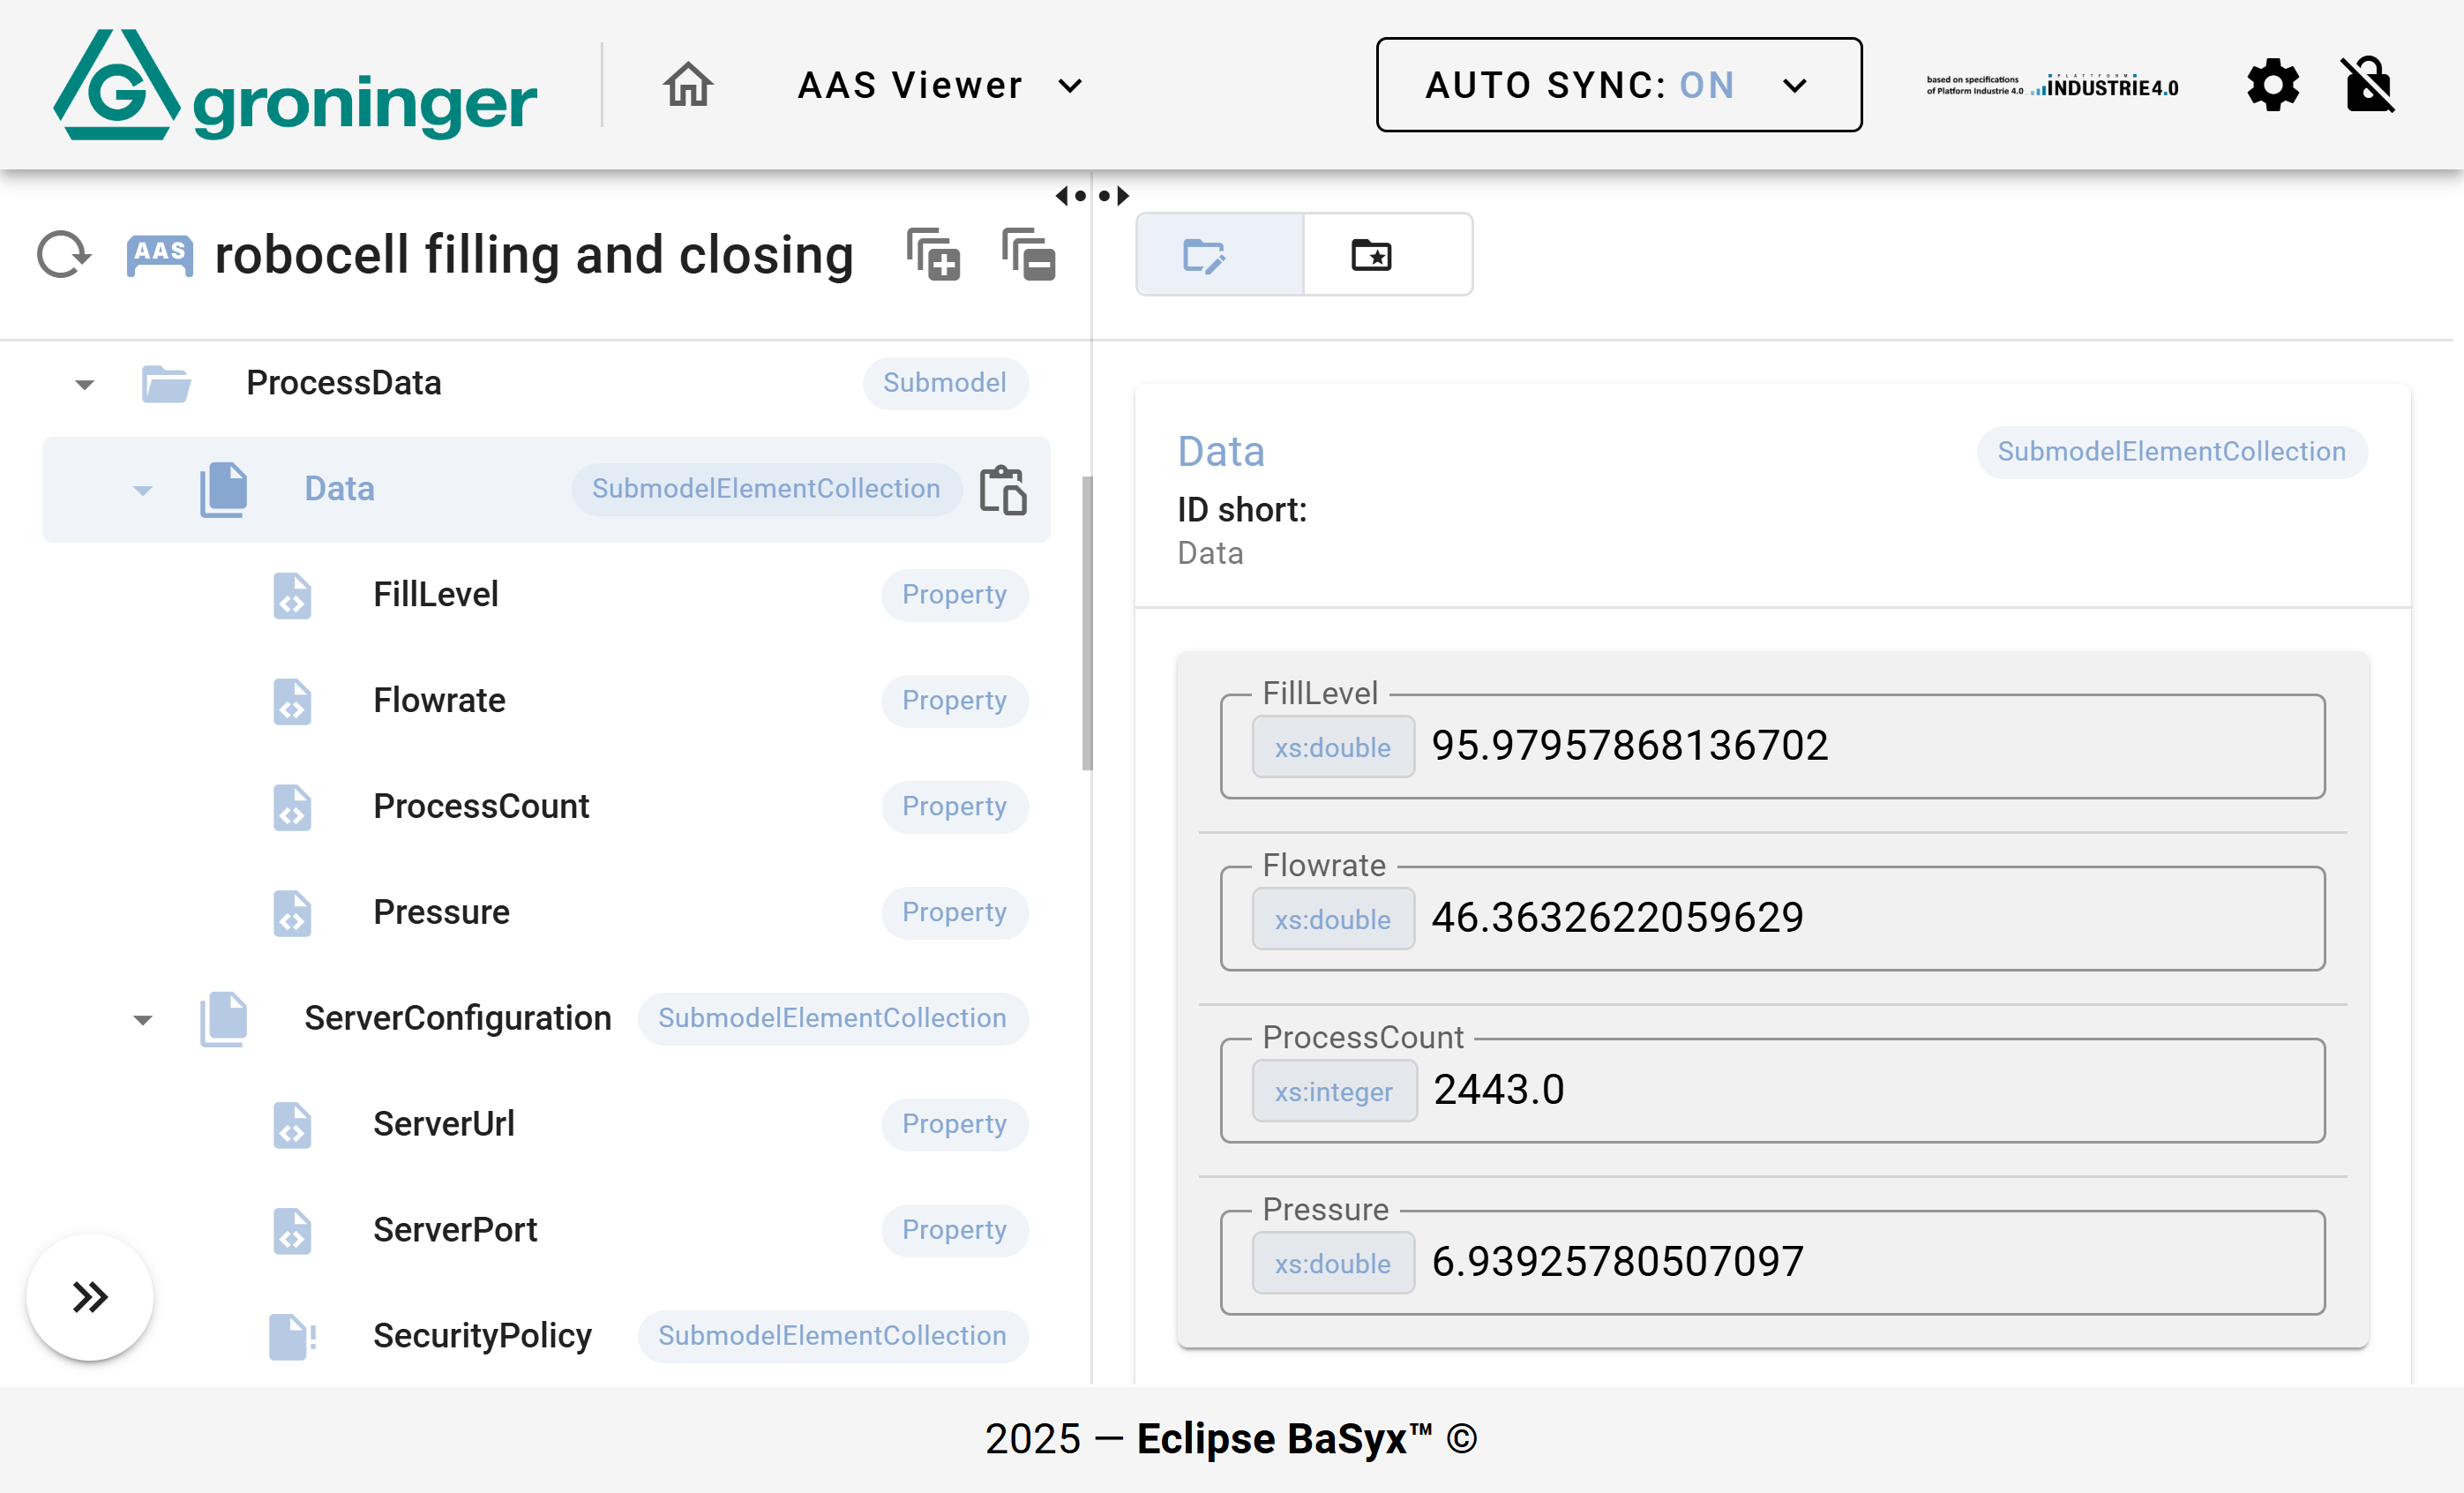
\includegraphics[width=1\textwidth]{Bilder/ErgebnisseAASWebUI/ProcessData.png}
    \caption{AAS Web UI: Prozessdaten}
    \label{fig:Processdata}
\end{figure}
\vspace{-0.5em}

Die Visualisierung der Prozessdaten erfolgt in der klassischen Elemente-Ansicht der AAS Web UI, wie in Abbildung~\ref{fig:Processdata} dargestellt, oder über ein speziell entwickeltes Plugin.
Damit die Werte in der Benutzeroberfläche aktuell bleiben, kann eine Synchronisationsfunktion aktiviert werden.
Dabei ruft die Weboberfläche die relevanten Daten in festen Intervallen, beispielsweise alle vier Sekunden, automatisch vom Repository ab.

Die Umsetzung ist protokolloffen und könnte grundsätzlich auf weitere Kommunikationsstandards wie \acs{mqtt} oder \acs{rest} erweitert werden.
Eine automatische bidirektionale Kommunikation, etwa das Zurückschreiben von Werten aus der \acs{aas} in externe Systeme, ist mit der eingesetzten Databridge derzeit jedoch nicht möglich.

\subsubsection*{Kontrollkomponente}
Das Submodell Kontrollkomponente dient der Abbildung und Visualisierung des aktuellen Maschinenstatus sowie der unterstützten Betriebsmodi.
Die Zustandsinformationen stammen aus dem Maschinensimulator, der sie in numerischer Form über einen \acs{opcua}-Server bereitstellt.
Über die Databridge werden diese Werte in nahezu Echtzeit in die \acs{aas} übertragen.
Vor der Speicherung erfolgt eine semantische Umwandlung mithilfe von JSONata, um die numerischen Codes in sprechende Zustandsbezeichnungen zu überführen.

Die Zustände orientieren sich am PackML-Standard (Packaging Machine Language), einem von der OMAC (Organization for Machine Automation and Control) entwickelten Modell zur einheitlichen Beschreibung von Maschinenzuständen und zulässigen Zustandsübergängen, insbesondere für Verpackungsmaschinen \cite{OMAC}. 
Der Standard definiert insgesamt 17 Maschinenzustände und legt fest, welche Übergänge zwischen diesen möglich sind. 
Dieses Konzept kommt auch bei der robocell-Linie zum Einsatz und ermöglicht eine konsistente und interoperable Erfassung des Maschinenstatus über verschiedene Systeme hinweg.

Die Visualisierung erfolgt über ein in die AAS Web UI integriertes Vue.js-Plugin, das den Maschinenstatus als PackML-Zustandsautomat darstellt.
Das Plugin basiert auf einer Entwicklung der Hochschule für Technik und Wirtschaft Berlin \cite{HTW1, HTW2} und wurde funktional angepasst, um es in die AAS Web UI zu integrieren und die im Demonstrator benötigten Steuer- und Anzeigeoptionen zu unterstützen.

Abbildung~\ref{fig:PackMLZustandsautomat} zeigt die Darstellung des Zustandsautomaten in der Benutzeroberfläche.
Damit Statusänderungen unmittelbar sichtbar werden, ist eine Polling-Logik implementiert, die den aktuellen Maschinenstatus in festen Intervallen aus dem Submodel Repository der AAS Environment abruft und im Zustandsautomaten aktualisiert.

Neben der reinen Statusanzeige erlaubt das Plugin auch die Steuerung zulässiger Zustandsübergänge direkt aus der Benutzeroberfläche heraus.
Befindet sich die Maschine beispielsweise im Zustand Execute, können Befehle wie Stop, Hold, Suspend oder Abort ausgelöst werden.
Darüber hinaus lässt sich der Betriebsmodus (Produktion, Manuell oder Wartung) setzen, der ebenfalls als Property im Submodell verwaltet wird.

\newpage
\begin{figure}[htbp]
    \centering 
    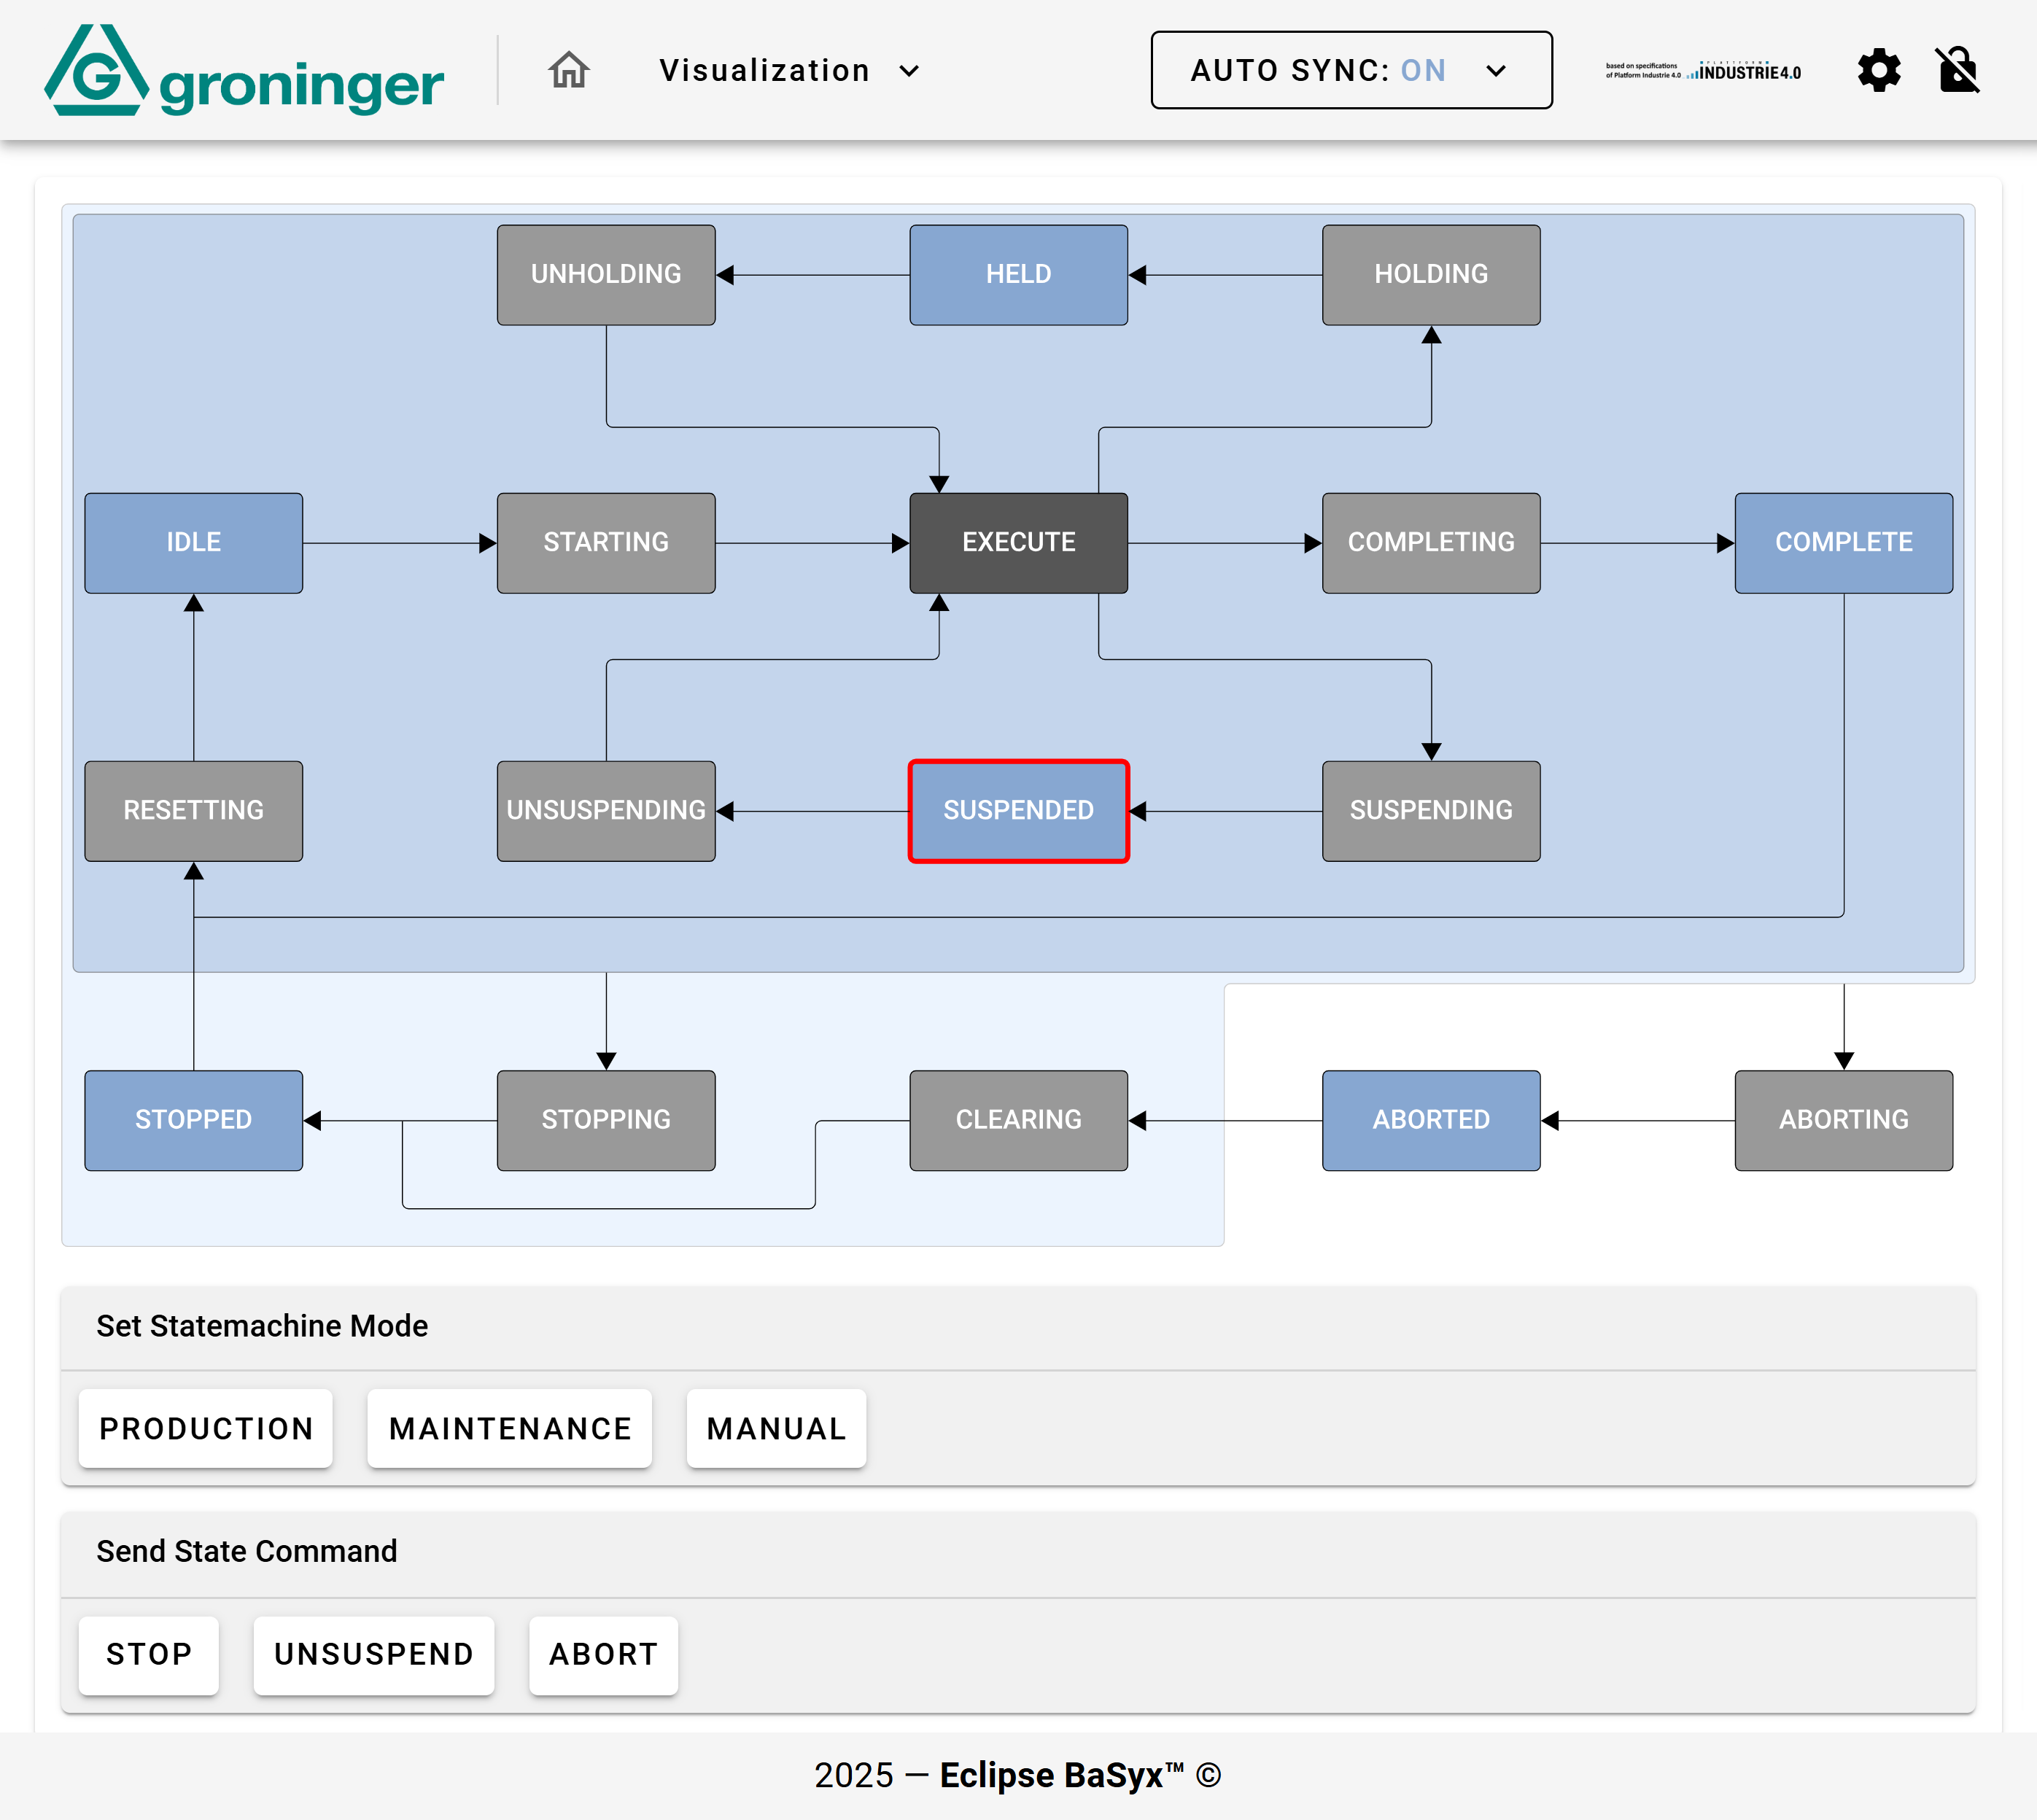
\includegraphics[width=1\textwidth]{Bilder/ErgebnisseAASWebUI/Kontrollkomponente.png} 
    \caption{AAS Web UI: PackML-Zustandsautomat} 
    \label{fig:PackMLZustandsautomat} 
\end{figure}
\vspace{-0.5em}

Im Demonstrator werden Befehle direkt per WebSocket an den Maschinensimulator übermittelt und dort ohne weitere Prüfungen übernommen. 
Dadurch entsteht eine direkte Feedback-Schleife zwischen der \acs{aas} und dem simulierten Asset.
In einer realen Maschine würden diese Signale hingegen zunächst über ein geeignetes Industrieprotokoll wie \acs{opcua} an die speicherprogrammierbare Steuerung (SPS) übertragen und dort validiert werden müssen, bevor der neue Zustand an die \acs{aas} zurückgemeldet wird.

\subsubsection*{Zeitreihendaten}
Das Submodell Zeitreihendaten dient der Einbettung historischer Messwerte in die \acs{aas}. 
Im Demonstrator werden hierfür exemplarisch die Messgrößen Druck und Temperatur verwendet, die kontinuierlich vom \acs{opcua}-Server des Datengenerators bereitgestellt werden. 
Anstatt diese Werte direkt in der \acs{aas} abzulegen, werden sie mithilfe von Telegraf in eine externe InfluxDB-Datenbank übertragen. 
Telegraf abonniert dazu die relevanten Variablen des \acs{opcua}-Servers und schreibt geänderte Werte unmittelbar in die Datenbank.

Die Anbindung an die \acs{aas} erfolgt über ein LinkedSegment (eine \acs{smc}) im Submodell, das alle für die Datenabfrage erforderlichen Parameter enthält, wie den Endpunkt der InfluxDB und die zugehörige Abfragebeschreibung. 
Dadurch können Anwendungen, die auf die \acs{aas} zugreifen, die Zeitreihendaten gezielt abrufen, ohne Details zur technischen Implementierung der Datenbank kennen zu müssen.

Zur Visualisierung steht in der AAS Web UI ein spezielles Plugin zur Verfügung, das auf die im LinkedSegment hinterlegten Parametern zugreift und Abfragen an die InfluxDB stellt. 
Ein Nutzer kann dabei auswählen, ob einzelne Messgrößen oder kombinierte Ansichten mehrerer Werte angezeigt werden sollen. 
Abbildung~\ref{fig:LiniendiagrammBaSyx} zeigt exemplarisch ein Liniendiagramm mit den zeitlichen Verläufen von Druck und Temperatur über einen Zeitraum von fünf Minuten.

\begin{figure}[htbp]
    \centering
        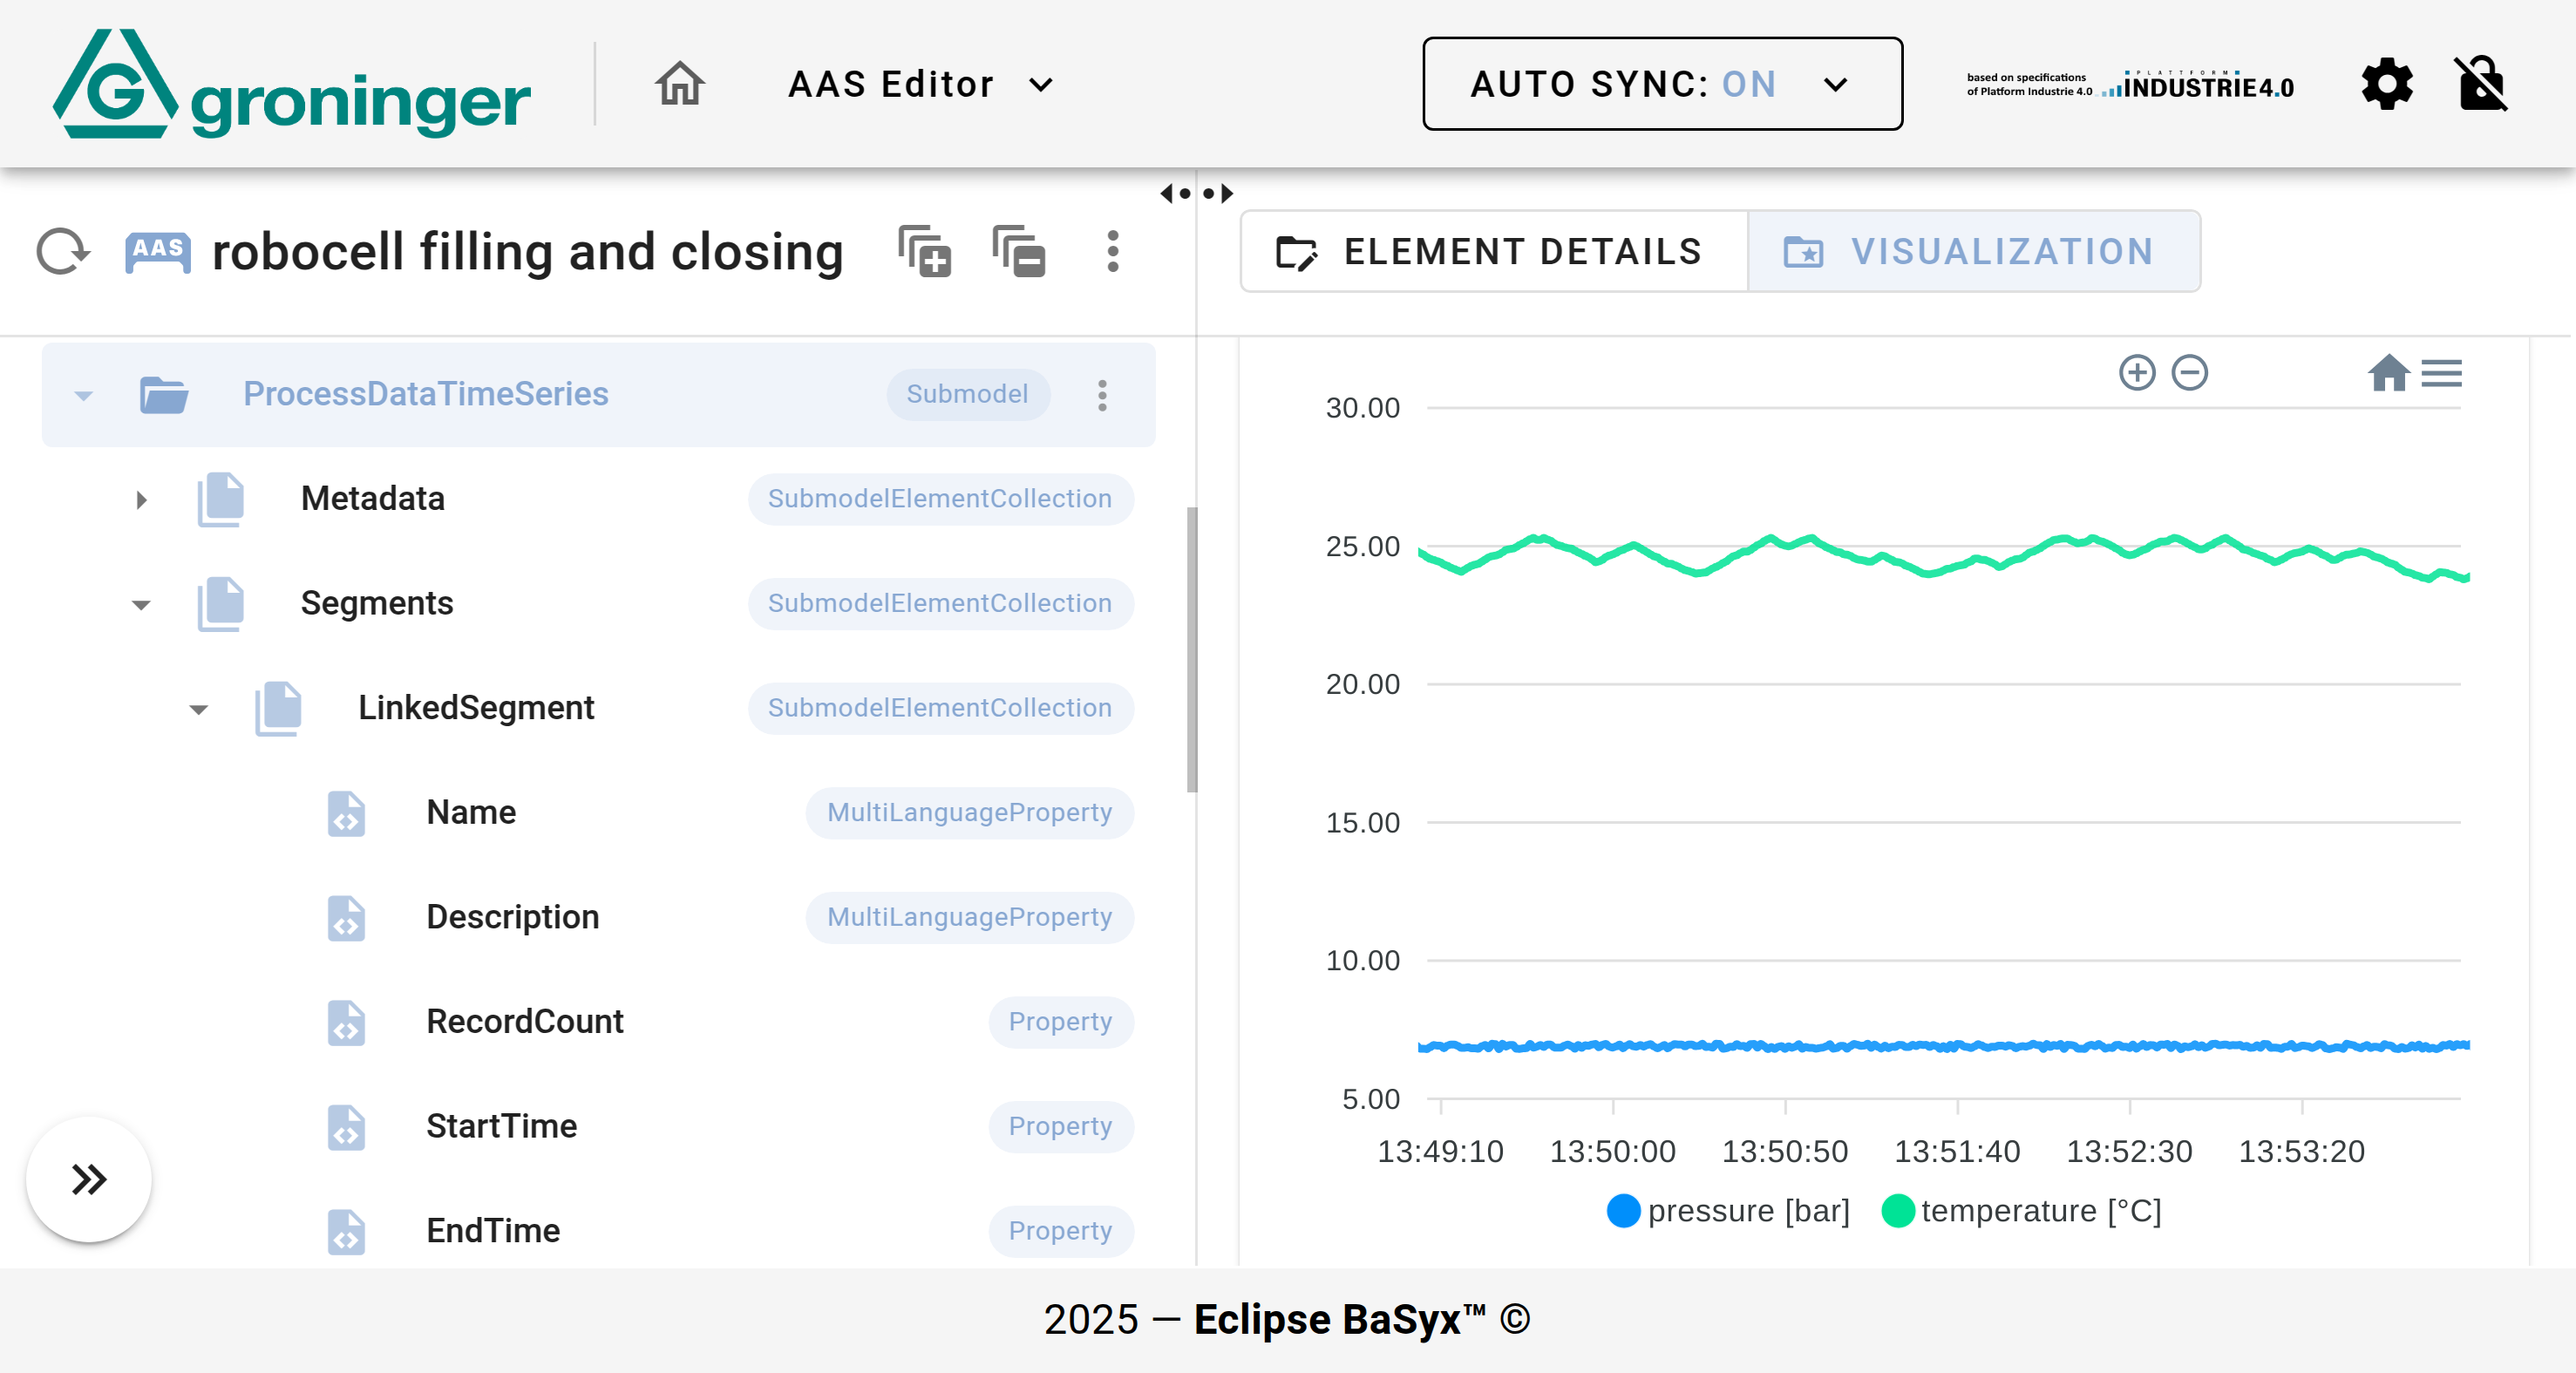
\includegraphics[width=1\textwidth]{Bilder/ErgebnisseAASWebUI/Zeitreihen.png}
    \caption{AAS Web UI: Zeitreihendaten (Liniendiagramm)}
    \label{fig:LiniendiagrammBaSyx}
\end{figure}
\vspace{-0.5em}

Ein wesentlicher Vorteil dieser Umsetzung liegt in der Entkopplung von Datenspeicherung und \acs{aas}. 
Da die \acs{aas} selbst nicht für die Ablage großer oder historischer Datenmengen ausgelegt ist, ermöglicht die Auslagerung in eine externe Zeitreihendatenbank eine effiziente Speicherung und Verarbeitung. 
Zudem können die Daten durch die strukturierte Referenzierung über das LinkedSegment einfach in weiteren Anwendungen, wie Analysesystemen oder KI-gestützten Verfahren, weiterverwendet werden.

\subsubsection{Herausforderungen bei der Implementierung}
Im Rahmen der Implementierung des Demonstrators traten verschiedene Herausforderungen auf, die sowohl technische als auch methodische Aspekte betrafen. 
Diese ergaben sich unter anderem aus der noch jungen Verbreitung der \acs{aas} im Maschinenbau, der eingeschränkten Datenverfügbarkeit sowie den Limitierungen der eingesetzten Werkzeuge. 
Die wesentlichen Punkte sind im Folgenden zusammengefasst:

\begin{enumerate}
    \item \textbf{Fehlende praxisnahe Vorlagen für den Maschinenbau:}  
    Zwar existieren bereits diverse \acsp{smt}, Spezifikationen sowie allgemeine Anwendungsfälle, diese sind jedoch primär auf Komponentenhersteller ausgerichtet.  
    Konkrete Vorlagen und praxisnahe Anwendungsfälle, die speziell auf den Maschinenbau und die Anforderungen des Demonstrators zugeschnitten sind, standen jedoch nur begrenzt zur Verfügung.

    \item \textbf{Begrenzte Datenverfügbarkeit:}  
    Da keine reale Maschine angebunden war, mussten Echtzeitdaten simuliert werden.  
    Zudem waren nicht alle relevanten Daten im PLM-System so dokumentiert, dass eine direkte Übernahme möglich gewesen wäre.  
    Viele Informationen mussten daher manuell aus verschiedenen Dokumenten, wie der Betriebsanleitung, extrahiert werden.  

    \item \textbf{Begrenzte Verfügbarkeit semantischer Beschreibungen:}  
    Für viele spezifische Maschineneigenschaften, wie technische Parameter im Verarbeitungsbereich (z.\,B. Spritze, Vial, Zylinderampulle) und deren Detailwerte (z.\,B. Füllmenge, Stopfenhöhe), existieren bislang keine standardisierten ECLASS-Beschreibungen.  
    Diese mussten daher manuell angelegt werden, was zeitaufwendig war und die Interoperabilität einschränkt.

    \item \textbf{Eingeschränkte Funktionalität der eingesetzten Tools:}  
    Die verwendeten Werkzeuge unterstützten nicht alle benötigten Funktionen.  
    So wurden beispielsweise beim Hochladen von Dateien in der AAS Web UI keine Einträge im Discovery Service erzeugt.  
    Da diese Funktionalität erforderlich war, musste sie mithilfe eines eigens entwickelten Skripts ergänzt werden.  
    Eine detaillierte Evaluierung der eingesetzten Tools erfolgt in Kapitel~XY.

    \item \textbf{Inkonsistenzen zwischen Spezifikationen und Tools:}  
    \acsp{smt} und die zugehörigen Spezifikationen wiesen teilweise Inkonsistenzen auf, etwa unterschiedliche Werte in der Dokumentation im Vergleich zu den AASX-Vorlagen.  
    Dies führte dazu, dass einige Plugins nicht oder nur eingeschränkt funktionierten, da sie auf korrekte semantische Beschreibungen angewiesen sind.  
    Die Fehlerbehebung erforderte eine manuelle Anpassung der \acsp{smt}, was zusätzlichen Aufwand verursachte.
\end{enumerate}

\newpage
\subsection{KI-Modell zur Anomalieerkennung}

Für die Anomalieerkennung wurde der zuvor trainierte Autoencoder im Evaluierungsmodus eingesetzt, sodass während der Auswertung keine Anpassungen der Modellparameter erfolgen.
Die Testdaten basieren, wie beim Training, auf simulierten Temperaturverläufen aus dem Datengenerator, die analog zu den Zeitreihendaten in Kapitel \ref{sec:DynamischeSubmodelle} in einer InfluxDB gespeichert wurden.

Als Eingabe erhält das Modell kurze Sequenzen von jeweils fünf Messwerten.
Im Unterschied zur Trainingsphase enthalten die Testdaten gezielt eingefügte Anomalien, um die Erkennungsfähigkeit des Modells zu prüfen.
Dabei wurden vier Anomalietypen simuliert: dauerhaft erhöhte Werte, ein einzelner ausgeprägter Peak, ein linearer Anstieg über mehrere Zeitpunkte sowie invertierte Werte im Vergleich zum Normalverlauf.

Während der Auswertung berechnet der Autoencoder für jede Sequenz den Rekonstruktionsfehler als durchschnittliche Abweichung zwischen Eingabe- und Ausgabedaten. 
Zur Klassifikation dient ein Schwellenwert, der aus dem Mittelwert des Fehlers plus dem Zweifachen der Standardabweichung gebildet wird. 
Überschreitet der Fehler einer Sequenz diesen Wert, wird das gesamte Zeitfenster als Anomalie markiert.

Zur Veranschaulichung werden zwei Beispiele gezeigt, die unterschiedliche Anomalietypen repräsentieren. 
Abbildung~\ref{fig:Fall1} zeigt einen Temperaturverlauf mit dauerhaft erhöhten Werten im Bereich t = 10000 - 10010 (gezielt eingefügte Anomalie). 
Das Modell erkennt die Anomalie zuverlässig, allerdings leicht verzögert. 
Dies liegt an der Mittelwertbildung über das Fünf-Werte-Fenster.
Erst wenn mehrere aufeinanderfolgende Werte vom Normalverlauf abweichen, steigt der Fehler ausreichend an.

\begin{figure}[htbp]
    \centering
        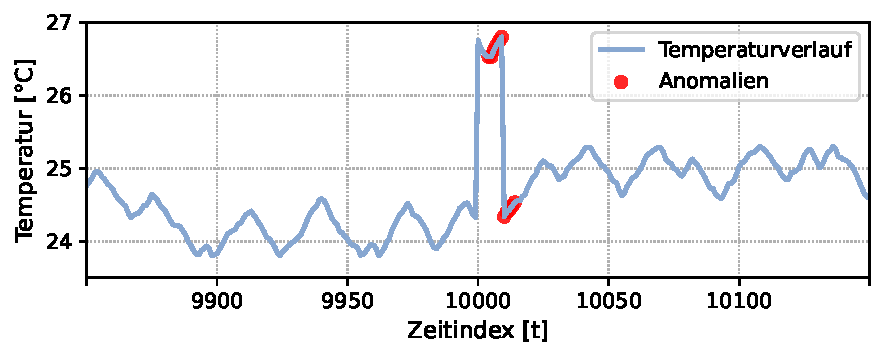
\includegraphics[width=1\textwidth]{Bilder/Ergebnisse/KI/Fall1.pdf}
        \vspace{-2em}
    \caption{Anomalieerkennung Fall 1: Überhöhte Daten}
    \label{fig:Fall1}
\end{figure}
\vspace{-0.5em}

In Abbildung~\ref{fig:Fall2} ist ein Temperaturverlauf mit einem gleichmäßigen, linearen Anstieg im Bereich t = 25343 - 25393 (gezielt eingefügte Anomalie) dargestellt. 
Auch hier klassifiziert das Modell den Verlauf korrekt als Anomalie. 
Dies zeigt, dass die Erkennung nicht nur auf plötzliche Ausreißer reagiert, sondern auch schleichende Veränderungen im Signalverlauf erkennt.


\begin{figure}[htbp]
    \centering
        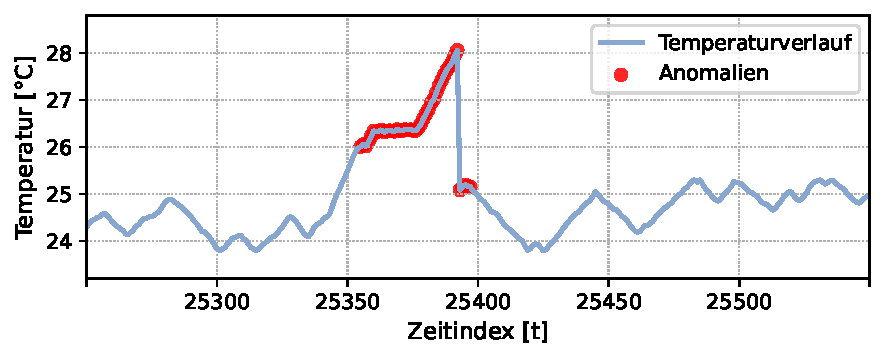
\includegraphics[width=1\textwidth]{Bilder/Ergebnisse/KI/Fall2.pdf}
        \vspace{-2em}
    \caption{Anomalieerkennung Fall 2: Linearer Anstieg}
    \label{fig:Fall2}
\end{figure}
\vspace{-0.5em}

In allen Testfällen mit künstlich erzeugten Anomalien erfolgte die Klassifikation korrekt, ohne Fehlalarme. 
Aufgrund der Fenstergröße und der Mittelwertbildung tritt die Markierung jedoch häufig leicht verzögert auf, wodurch einzelne Sequenzen innerhalb einer Anomaliephase nicht als abweichend markiert werden. 
Da ausschließlich synthetische Abweichungen geprüft wurden, ist zu erwarten, dass reale Anomalien aufgrund ihrer höheren Komplexität eine größere Herausforderung darstellen.

Zur Verbesserung könnten umfangreichere und variantenreichere Trainings- und Testdaten eingesetzt werden. 
Auch leistungsfähigere Architekturen wie tiefere Autoencoder oder LSTM-basierte Netze (Long Short-Term Memory, eine spezielle Form rekurrenter neuronaler Netze zur Verarbeitung von Zeitreihen) bieten Potenzial, zeitliche Abhängigkeiten präziser zu erfassen.
Diese Ansätze wurden aufgrund begrenzter Rechenressourcen im Rahmen dieser Arbeit nicht weiterverfolgt, können aber eine Grundlage für zukünftige Entwicklungen bilden.

Dennoch zeigt sich, dass das gewählte Konzept grundsätzlich umsetzbar ist und sich für eine Einbettung in industrielle Szenarien eignet. 
In Verbindung mit realen Maschinendaten können erkannte Anomalien genutzt werden, um proaktive Wartungsmaßnahmen einzuleiten. 
Dadurch ließe sich die Anlagenverfügbarkeit erhöhen und ungeplante Stillstandszeiten verringern.
Werden neben Sensordaten zusätzlich technische Stammdaten oder standardisierte Beschreibungen berücksichtigt, wie sie auch im AAS-Demonstrator hinterlegt sind, wird eine noch umfassendere Analyse möglich, die zugleich die Grundlage für weiterführende Predictive-Maintenance-Ansätze bilden könnte.

\newpage
\subsection{Anwendungsfall Digitaler Produktpass}
Der Anwendungsfall Digitaler Produktpass demonstriert, wie Nachhaltigkeitsinformationen in Form von \acs{pcf}-Werten direkt in der AAS einer Maschine abgebildet werden können.
Grundlage bildet der in Kapitel \ref{sec:AAS-Demonstrator} vorgestellte AAS-Demonstrator, der zu diesem Zweck um ein Submodell zur Abbildung des \acs{cf} erweitert wurde.
Neben der dynamischen Berechnung und Aggregation dieser Werte wird im Folgenden auch dargestellt, wie der Zugriff auf die im DPP enthaltenen Informationen durch unterschiedliche Nutzerrollen und technische Clients geregelt ist.

\subsubsection{Abbildung des PCF}
Das CF-Submodell bildet die Lebenszyklusphasen Material, Produktion und Cradle to Gate jeweils in eigenen \acsp{smc} ab.
Abbildung~\ref{fig:SubmodellCF} zeigt exemplarisch die \acs{smc} für die Phase Cradle to Gate (links) sowie die integrierte Komponentenliste (rechts), in der die für die Berechnung herangezogenen Siemens-Komponenten hinterlegt sind.

\begin{figure}[htbp]
    \centering
        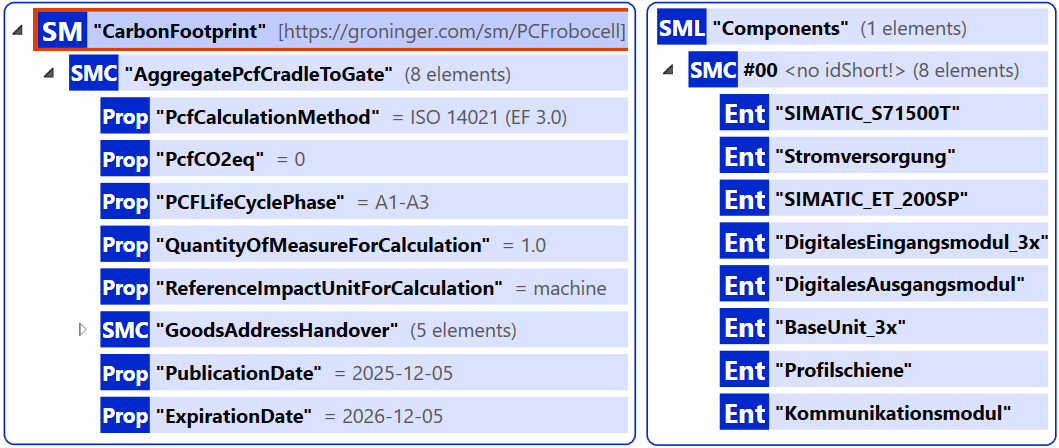
\includegraphics[width=1\textwidth]{Bilder/ErgebnissePackageExplorer/CarbonFoorprintTest.png}
    \caption{CF-Submodell der robocell}
    \label{fig:SubmodellCF}
\end{figure}

Die Aggregation der CO\textsubscript{2}-Äquivalente erfolgt dynamisch über einen Microservice. 
Dieser ist als Docker-Container implementiert und greift über die REST-Schnittstellen des BaSyx-Backends auf die in der Komponentenliste hinterlegten Entitäten zu. 
Mithilfe des Discovery Service werden deren AAS identifiziert und vorhandene CF-Submodelle ausgelesen. 
Die enthaltenen PCF-Werte werden anschließend zu Gesamtwerten für die einzelnen Lebenszyklusphasen aggregiert und in das CF-Submodell der Haupt-AAS zurückgeschrieben.

Die Berechnung kann direkt über ein Plugin in der AAS Web UI ausgelöst werden.
 Nach Abschluss des Berechnungsprozesses werden die aktualisierten Werte automatisch vom Submodel Repository abgefragt und in der Benutzeroberfläche aktualisiert.
Abbildung~\ref{fig:PluginAggregation} zeigt die entsprechende Visualisierung: links die aggregierten CO\textsubscript{2}-Äquivalente, rechts die zugehörigen Lebenszyklusphasen.

\begin{figure}[htbp]
    \centering
        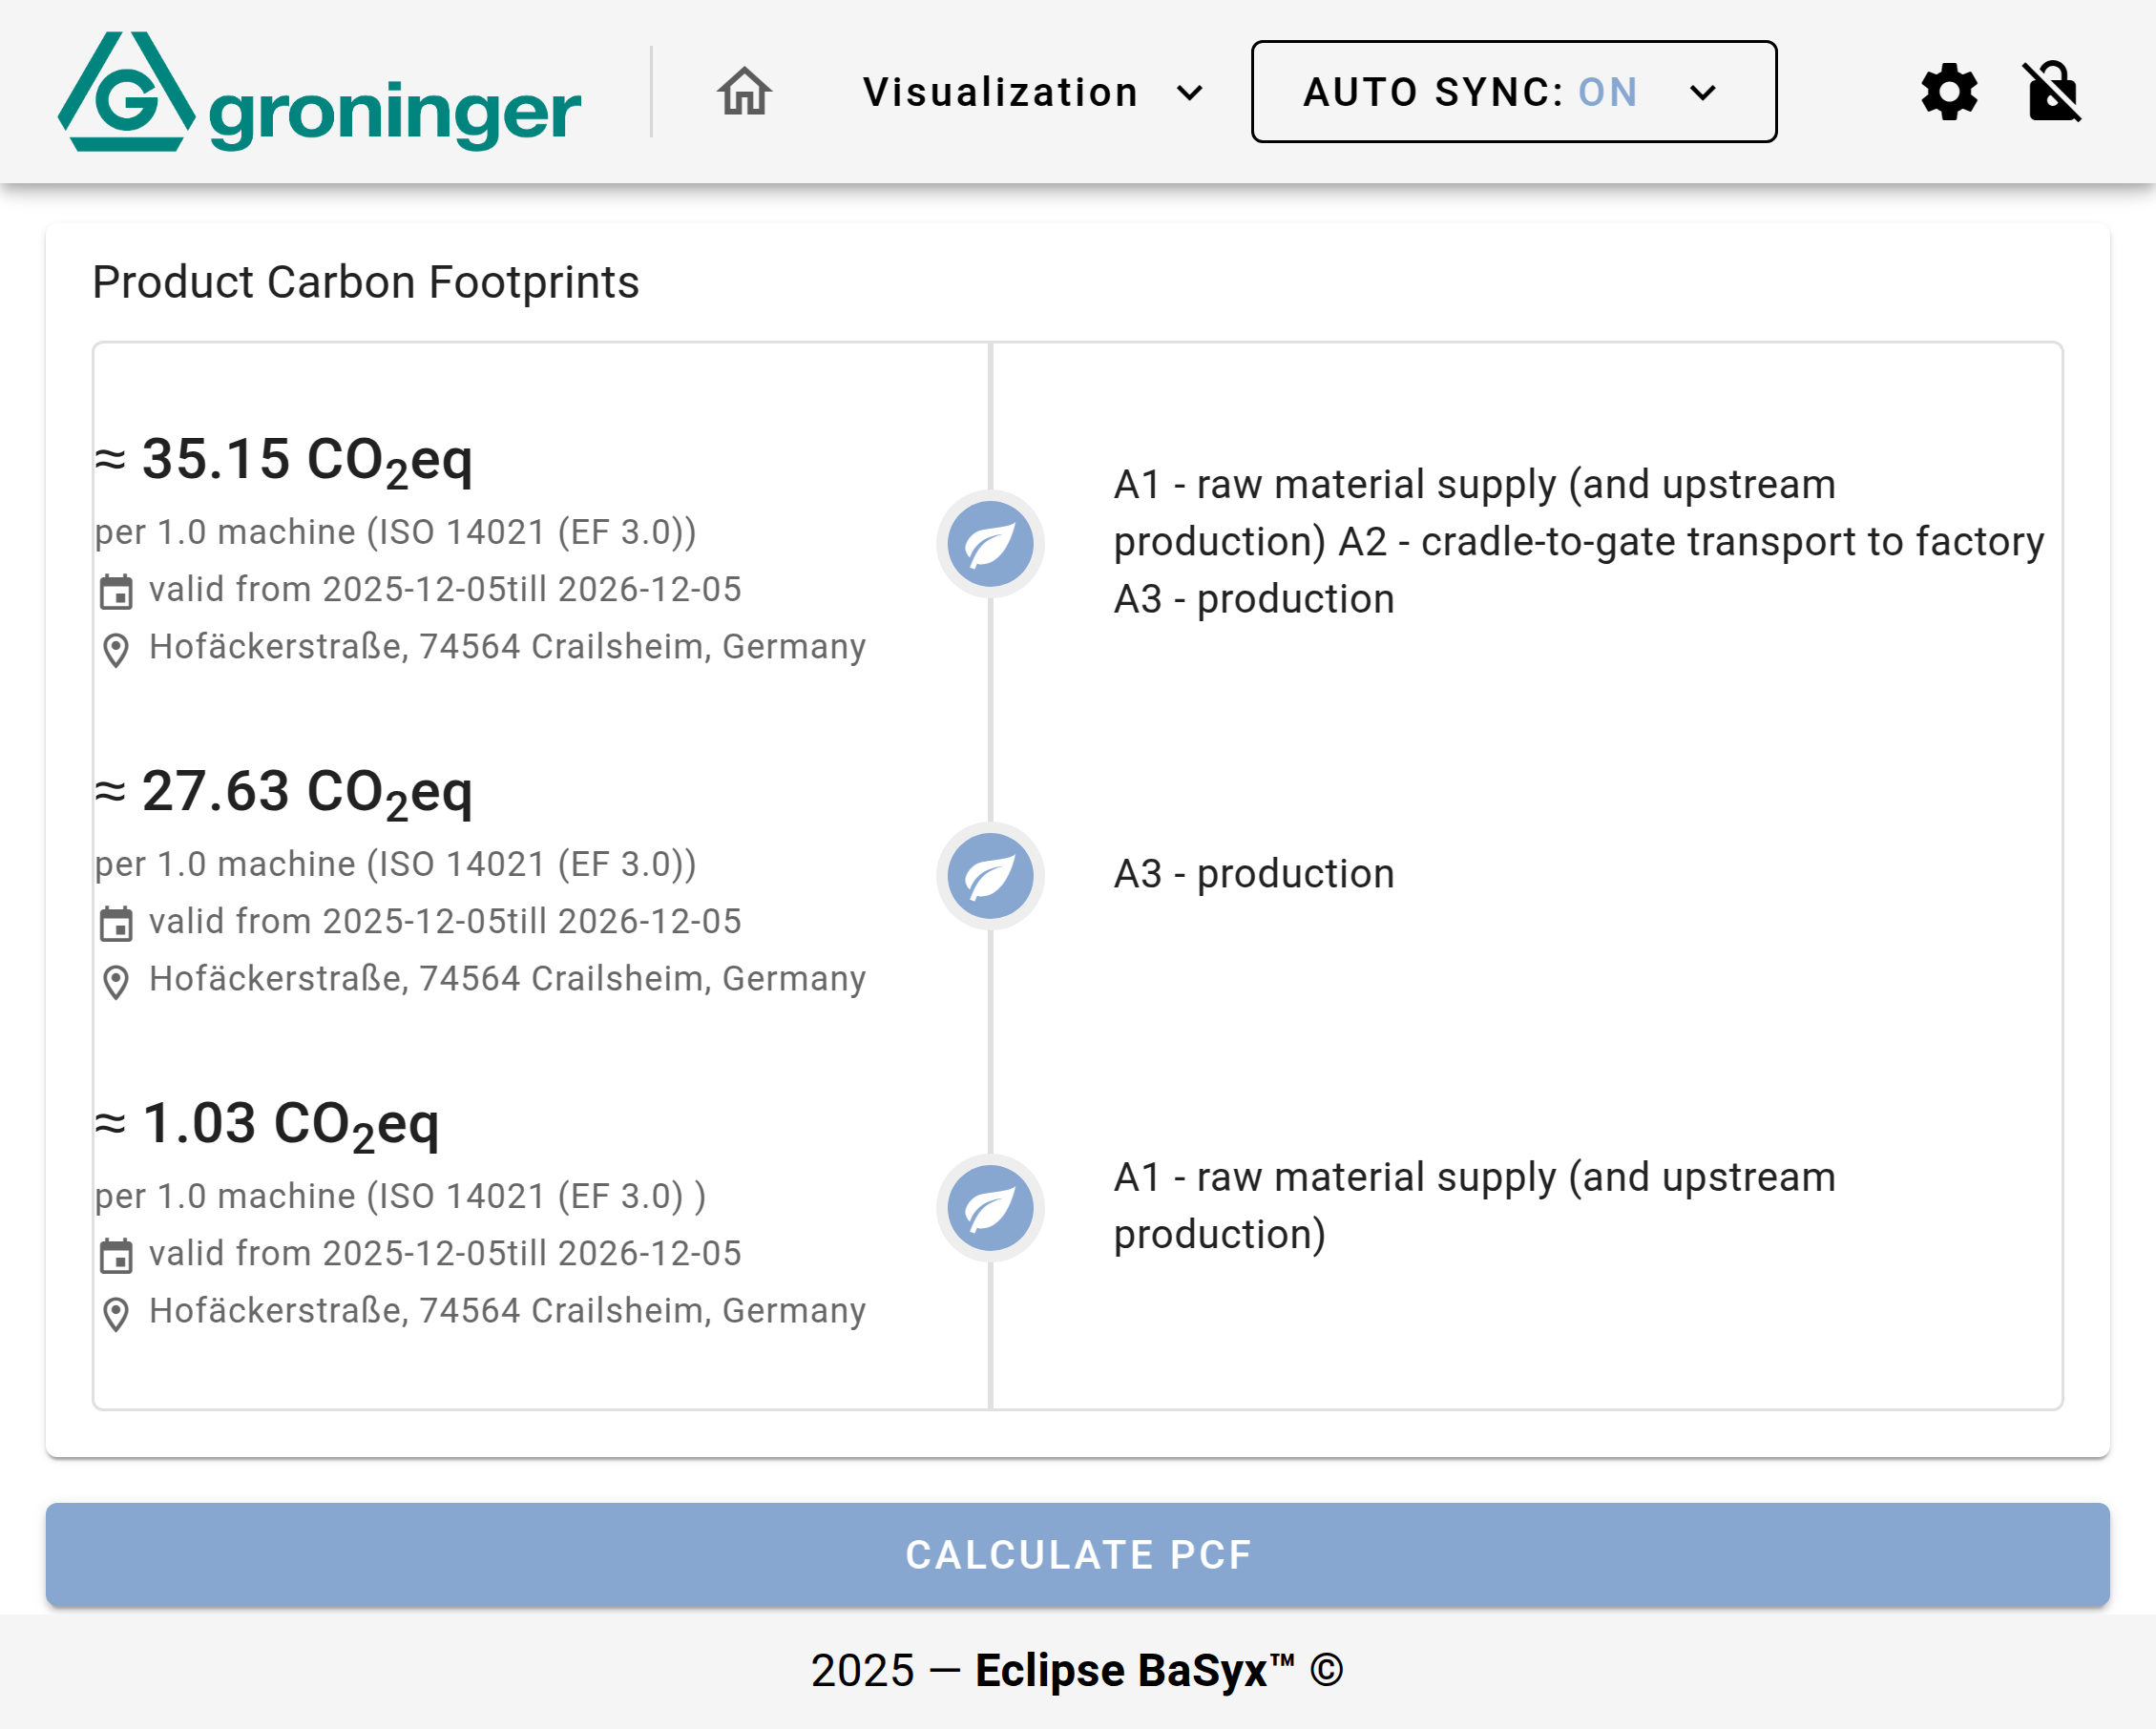
\includegraphics[width=1\textwidth]{Bilder/ErgebnisseAASWebUI/CarbonFootprint.png}
    \caption{Visualisierung der aggregierten PCF-Werte}
    \label{fig:PluginAggregation}
\end{figure}

Der Ansatz ist flexibel erweiterbar.
Bei Verfügbarkeit weiterer Komponenten-AAS lässt sich die Liste unkompliziert ergänzen, sodass sukzessive die gesamte Maschine berücksichtigt werden kann. 
Perspektivisch ist auch eine Erweiterung auf weitere Lebenszyklusphasen, wie Nutzung oder Entsorgung, sowie die Einbeziehung des TCF denkbar, um eine ganzheitliche ökologische Bilanzierung zu ermöglichen.

\subsubsection{Rollenbasierter Zugriff auf Submodelle}
Der digitale Produktpass wird im Demonstrator durch die erweiterte AAS der robocell-Maschine repräsentiert. 
Um sensible Inhalte gezielt und sicher bereitzustellen, wurde eine rollenbasierte Zugriffskontrolle implementiert. 
Die Authentifizierung und Autorisierung erfolgt über Keycloak, das als Docker-Container in die BaSyx-Architektur integriert ist.

Exemplarisch wurden drei Nutzer mit zugehörigen Rollen eingerichtet, deren Rechte in separaten Konfigurationsdateien für die jeweiligen BaSyx-Dienste hinterlegt sind.

\newpage
\begin{itemize}[noitemsep, leftmargin=*, label=\textbullet]
  \item \makebox[6cm][l]{\textbf{groninger.meyer}} (Rolle: \textit{Groninger-Mitarbeiter})
    \begin{itemize}[noitemsep, leftmargin=2em, label=--]
      \item uneingeschränkter Zugriff auf alle Submodelle
    \end{itemize}
  \item \makebox[6cm][l]{\textbf{customer.doe}} (Rolle: \textit{Kunde})
    \begin{itemize}[noitemsep, leftmargin=2em, label=--]
      \item Zugriff auf ausgewählte Submodelle (z.\,B. Typenschild, CF)
    \end{itemize}
  \item \makebox[6cm][l]{\textbf{technician.john}} (Rolle: \textit{Service-Techniker})
    \begin{itemize}[noitemsep, leftmargin=2em, label=--]
      \item Lese- und Schreibrechte auf wartungsrelevante Submodelle
    \end{itemize}
\end{itemize}
\vspace{0.5em}

Eine Möglichkeit zur Einsicht der im \acs{dpp} enthaltenen Informationen bietet die AAS Web UI.
Ist \acs{rbac} aktiviert, wird der Benutzer beim Aufruf der Oberfläche automatisch zur Keycloak-Anmeldeseite weitergeleitet.
Wie in Abbildung~\ref{fig:KeycloakAnmeldeSeite} dargestellt, erfolgt die Authentifizierung über die in Keycloak hinterlegten Zugangsdaten.

\begin{figure}[htbp]
    \centering
        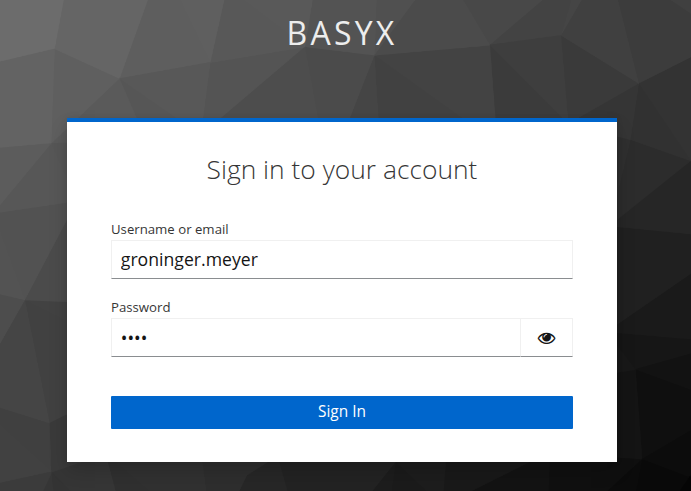
\includegraphics[width=0.7\textwidth]{Bilder/Ergebnisse/DPP/KeycloakAnmeldeSeite.png}
    \caption{Keycloak-Anmeldeseite für die AAS Web UI}
    \label{fig:KeycloakAnmeldeSeite}
\end{figure}

Nach erfolgreicher Anmeldung erhält die AAS Web UI ein Zugriffstoken mit den Rolleninformationen des Nutzers.
Dieses Token wird bei allen Anfragen an die BaSyx-Komponenten automatisch mitgesendet.
Die jeweiligen Dienste prüfen es gegen die hinterlegten \acs{rbac}-Regeln und entscheiden so über die tatsächliche Zugriffsberechtigung.

Meldet sich beispielsweise der Nutzer customer.doe an, so sieht er nur die für seine Rolle freigegebenen Submodelle. 
Andere Submodelle wie Kontrollkomponente oder Wartung bleiben verborgen. 
Zudem besitzt er ausschließlich Leserechte, das heißt Änderungsversuche werden mit einem Fehler abgelehnt.

Neben der AAS Web UI ist auch ein direkter Zugriff auf die BaSyx-Komponenten über die REST-API möglich, der insbesondere für technische Clients relevant ist. 
Dafür wurden in Keycloak drei Clients mit Service Accounts angelegt, die denselben Rollen wie die Benutzerkonten entsprechen und somit identische Berechtigungen besitzen.

Zur Validierung der Konfiguration wurde Postman eingesetzt. 
Die Clients rufen dabei über den Token-Endpunkt von Keycloak Zugriffstokens ab und nutzen diese für API-Anfragen. 
Abbildung~\ref{fig:KeycloakAnmeldeSeite} zeigt exemplarisch eine DELETE-Anfrage des Service-Techniker-Clients. 
Da dieser nur Leserechte besitzt, wird die Anfrage mit HTTP 403 Forbidden abgelehnt. 
Mit dem Groninger-Client hingegen gelingt der Löschvorgang, da dessen Rolle uneingeschränkte Rechte umfasst (HTTP 204 No Content).

\begin{figure}[htbp]
    \centering
        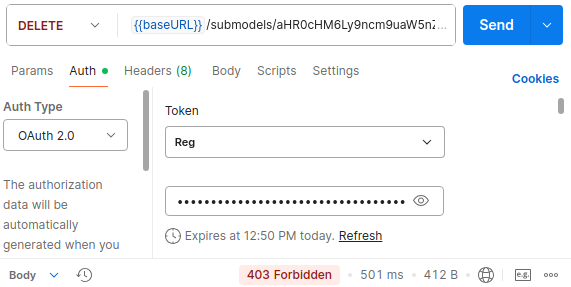
\includegraphics{Bilder/Ergebnisse/DPP/Postman/TechnicianDelet.png}
    \caption{DELETE-Anfrage des Service-Techniker-Clients in Postman}
    \label{fig:KeycloakAnmeldeSeite}
\end{figure}

Die Zugriffskontrolle mit BaSyx und Keycloak zeigt, dass sich Berechtigungen zuverlässig auf die AAS und ihre Submodelle übertragen lassen.
Dies bestätigt die Eignung der AAS als technische Grundlage für den \acs{dpp} und eröffnet Potenziale für Szenarien, in denen sensible Informationen, etwa Nachhaltigkeitsdaten, differenziert entlang der Wertschöpfungskette bereitgestellt werden.

\subsection{Anwendungsfall automatisierte Generierung der AAS}
Dieser Anwendungsfall demonstriert, wie sich AAS-Instanzen automatisiert erzeugen und in das BaSyx-System integrieren lassen.
Abbildung \ref{fig:AutomatisierteGenerierungAblauf} veranschaulicht den Ablauf.
Ausgangspunkt bildet ein unternehmensspezifisches Typ-Submodell, das mithilfe des Package Explorers aus dem SMT Generic Frame for Technical Data for Industrial Equipment in Manufacturing \cite{SpezifikaitonTechnischeDaten} abgeleitet wurde.
Dieses Template wird anschließend über ein Node.js-basiertes Mapping-Skript mit Beispieldaten ergänzt und in eine neue AAS-Instanz eingebettet.
Das Skript übernimmt auch die Registrierung im BaSyx-Backend, sodass die erzeugte AAS unmittelbar zur Verfügung steht und beispielsweise in der AAS Web UI visualisiert werden kann.

\begin{figure}[htbp]
    \centering
        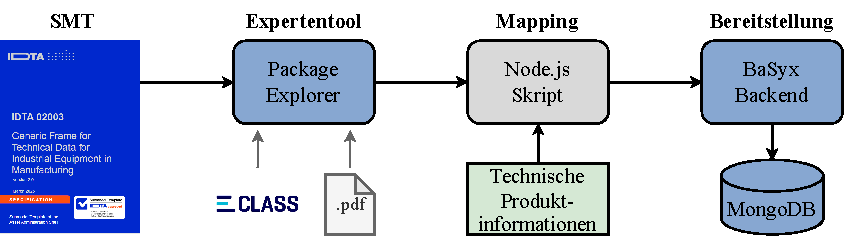
\includegraphics{Bilder/ErgebnisseAutomatisierteGenerierung/ARchitektur.pdf}
    \caption[Ablauf der automatisierten Generierung einer AAS]{Ablauf der automatisierten Generierung einer AAS (eigene Darstellung; Bildbestandteile: \cite{SpezifikaitonTechnischeDaten}, \cite{ECLASSLogo} )}
    \label{fig:AutomatisierteGenerierungAblauf}
\end{figure}

Der entwickelte Ansatz verdeutlicht, dass sich der manuelle Modellierungsaufwand im Package Explorer durch den teilautomatisierten Prozess erheblich reduzieren lässt. 
In diesem Anwendungsfall wurden zwar statische Beispieldaten eingesetzt, in einer produktiven Umgebung könnten jedoch die technischen Produktinformationen direkt aus bestehenden IT-Systemen übernommen werden. 
Bei groninger stammen diese primär aus dem PLM-System Agile. 
Eine entsprechende Anbindung war im Rahmen dieser Arbeit jedoch nicht umsetzbar.

Darüber hinaus ist der Prozess grundsätzlich auch auf weitere Submodelle übertragbar, sodass perspektivisch die AAS einer gesamten Maschine automatisiert erstellt werden könnte. 
Zudem wäre es möglich, die Mapping-Logik in eine Laufzeitumgebung zu integrieren. 
Dadurch ließe sich die Generierung, Bereitstellung und Aktualisierung von AAS-Instanzen vollständig automatisieren.

%Evaluation der eingesetzten Software
\subsection{Evaluierung eingesetzter Tools und Software}
Zur Umsetzung des AAS-Demonstrators sowie der zugehörigen Anwendungsfälle kamen zwei zentrale Softwarelösungen zum Einsatz.
Im Folgenden werden diese Werkzeuge hinsichtlich ihrer Funktionalität, Stärken und Schwächen evaluiert.
Die Bewertung stützt sich auf die Erfahrungen aus der praktischen Anwendung und berücksichtigt sowohl technische Aspekte als auch die Benutzerfreundlichkeit.

\newpage
\subsubsection{Package Explorer}

Der Package Explorer wurde während der gesamten Projektlaufzeit als zentrales Modellierungstool eingesetzt.
Er ermöglichte die Erstellung, Bearbeitung und Visualisierung von AAS einschließlich ihrer Submodelle und Submodellelemente.
Ein besonderer Vorteil war die Möglichkeit, semantische Beschreibungen direkt aus ECLASS-Katalogen zu importieren.
Dadurch verringerte sich der ansonsten sehr aufwendige manuelle Aufbau eigener Concept Descriptions deutlich, was den Modellierungsprozess spürbar beschleunigte.
Zudem überzeugte die benutzerfreundliche Oberfläche, die den Einstieg erleichterte, das Verständnis der AAS-Strukturen förderte und Verstöße gegen die Spezifikation der IDTA unmittelbar kenntlich machte.

In der praktischen Anwendung zeigten sich jedoch auch Einschränkungen.
Die integrierte Validierungsfunktion erwies sich als unzuverlässig, sodass zur Absicherung eine separate Test-Engine erforderlich war.
Während die Anbindung an den AASX Server Blazor problemlos funktionierte, war eine direkte Integration in modulare Laufzeitsysteme wie Eclipse BaSyx nicht möglich.
Die AAS mussten daher manuell bereitgestellt werden, was insbesondere bei einer größeren Anzahl oder häufigen Änderungen mit erheblichem Mehraufwand verbunden war.
Darüber hinaus wich der Package Explorer in einzelnen Punkten von den aktuellen AAS-Spezifikationen ab, was vereinzelt zu fehlerhaften semantischen Angaben führte, die nachträglich korrigiert werden mussten.

Insgesamt erwies sich der Package Explorer als hilfreiches Werkzeug für die statische Modellierung von AAS.
Die vorhandenen Exportfunktionen, insbesondere im AASX-Format, erleichterten die Weiterverwendung und Weitergabe maßgeblich.
Für automatisierte Szenarien bot das Tool hingegen nur eingeschränkte Unterstützung, die sich im Wesentlichen auf das Anlegen eigener \acsp{smt} beschränkte.

\newpage
\subsubsection{Eclipse BaSyx}

Die Eclipse-BaSyx-Plattform bildete in diesem Projekt die zentrale Laufzeitumgebung für den Betrieb von AAS. 
Ein wesentlicher Vorteil war der modulare Aufbau, der die Umsetzung praxisnaher Industrieszenarien erlaubte und zugleich eine flexible Konfiguration einzelner Komponenten zuließ. 
Ebenso eröffneten die standardisierten REST-APIs einen direkten Zugriff auf die einzelnen Komponenten, der dank der integrierten Swagger-Dokumentation unmittelbar getestet und transparent nachvollzogen werden konnte. 
Darüber hinaus erleichterte die DataBridge die Anbindung unterschiedlicher Protokolle, insbesondere von OPC UA, wodurch eine dynamische Erweiterung der AAS und die Umsetzung dynamischer Submodelle möglich wurde.

Außerdem stand mit der AAS WebUI eine Benutzeroberfläche zur Verfügung, die sowohl die Darstellung als auch die Anpassung von AAS-Inhalten erlaubte. 
Besonders hervorzuheben ist, dass für zentrale Submodelle bereits spezialisierte Plugins bereitstanden. 
Aufgrund des Open-Source-Charakters ließen sich diese problemlos erweitern oder durch eigene Entwicklungen ergänzen, sodass auch weitere Submodelle integriert und projektspezifische Anforderungen berücksichtigt werden konnten. 
Als besonders hilfreich erwies sich zudem die Synchronisationsfunktion, die insbesondere in dynamischen Szenarien sicherstellte, dass die angezeigten Daten stets aktuell blieben.

Erste Satz kommt noch..
Aufgrund des ausgiebigen Systems erwies sich der initiale Konfigurationsaufwand hoch.
Dies zeigte sich auch beim Einreichten von \acs{rbac}, bei dem jede Komponente seperat eingerichtet werden musste.
Zudem gestalltete sich der Start des Systems in der Docker.-Umgebung als sehr zeitintensiv.
Einige Komponenten wiesen Wartezeiten von bis zu mehreren Minuten auf, was natürlich was bei Testläufen oder häufigen Änderungen hinderte


Trotz dieser Vorteile zeigten sich in der praktischen Anwendung auch Einschränkungen. 
Der initiale Konfigurationsaufwand erwies sich als hoch, insbesondere bei der Einrichtung des rollenbasierten Zugriffskontrollsystems (RBAC), das für jede einzelne Komponente separat konfiguriert werden musste. 
Hinzu kam, dass der Start des Gesamtsystems als Docker vlt sagen? vergleichsweise lange dauerte, da die einzelnen Services nacheinander hochgefahren wurden, was Wartezeiten von bis zu mehreren Minuten verursachte. 
UNd es ist so das einzelne Services schon fast 2 minuten gebraucht haben weis nicht genau
Dies erwies sich vor allem bei Testläufen oder häufigen Anpassungen als hinderlich. 
Ergänzend zeigte sich, dass Änderungen an eingebundenen AAS nicht immer zuverlässig übernommen wurden. So wurden etwa aktualisierte Concept Descriptions nicht automatisch aus dem Repository synchronisiert, was zu Inkonsistenzen führte und manuelle Nacharbeit erforderte.

Negativ:

komplex hoher Konfigurationsaufwadn.
Zeigte sich insbesondere bei RBAC wo für jede Komponente einzeln aufgesetzt
Weis nicht ob das relevant ist aber die Umgebun gbrauchte immer richtig lang zum starten also einzelnbe Services bis hin zu 100s das könnte ich natürlich auch noch nachschauen 
das ist natürlich ärgerlich wenn man änderungen vornimmt oder etwas testen will.
ergänzend nicht gesatrtet wenn aktualisierte AAS über das eingebundene Repository eingebunden, weil CDS besipielsweise nicht aktuaölisiert wurden



Absatz 3: wünschenswert Änderungen an der AAS anzeigen 
